\documentclass[a4paper]{article}
\usepackage[a4paper,top=2cm,bottom=2cm,left=2cm,right=2cm,marginparwidth=2cm]{geometry}
\usepackage{lmodern}
\usepackage{listings}
\usepackage{amsmath}
\usepackage{amssymb}
\usepackage{bm}
\usepackage{textpos}
\usepackage{tcolorbox}
\usepackage{graphicx}
\usepackage{pgf,tikz}
\usepackage{url}
\usetikzlibrary{arrows,automata}

\setlength{\parindent}{0em}
\setlength{\parskip}{0.3em}
\lstset{language=Python,upquote=true,basicstyle=\ttfamily\small,breaklines=true}

\begin{document}
\title{AICE3002/AICE6001 Laboratory Portfolio\\Investigation 3 -- Convolutions, Coordinates, and Transfer}
\author{Jonathon Hare \& Antonia Marcu\\\{j.s.hare, a.marcu\}@soton.ac.uk}
\date{2026--27}
\maketitle

This is the third of four individual investigations that make up the laboratory portfolio. It should be completed after the CNN and transfer-learning practical work. You should write up your results, answers, and findings succinctly, and submit your executable notebook alongside the report.

You should use \emph{no more than two sides of A4} for this investigation. Code need not be reproduced in full: include only short snippets needed to explain your method. This investigation is worth 10 marks.

\section{When convolutional inductive bias gets in the way}

In the lab exercise you built and trained a couple of CNNs for image classification. You're now going to try something different and build some CNNs for an image-to-vector regression task - in particular you're going to implement a network that takes an image of a scatter plot, and predicts the parameters of the line of best fit.

\begin{center}
    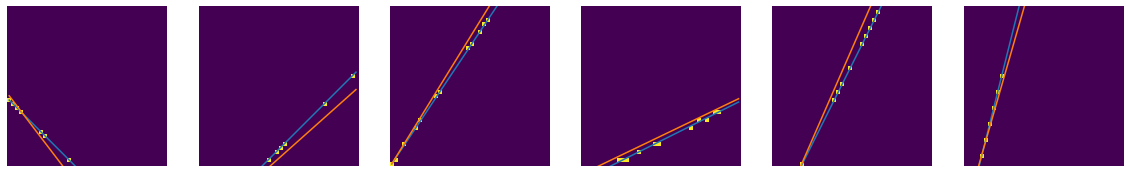
\includegraphics[width=0.82\textwidth]{plots.png}
\end{center}

The following code is used to generate the datasets for this task (get it in a useable form here: \url{https://gist.github.com/jonhare/73a59dcc5416729548a086a983e81f07}):

\begin{lstlisting}[language=Python]
import torch
from torchvision import transforms
from torch.utils.data import Dataset

class MyDataset(Dataset):
  def __init__(self, size=5000, dim=40, random_offset=0):
        super(MyDataset, self).__init__()
        self.size = size
        self.dim = dim
        self.random_offset = random_offset

  def __getitem__(self, index):
      if index >= len(self):
          raise IndexError('{} index out of range'.format(self.__class__.__name__))
      
      rng_state = torch.get_rng_state()
      torch.manual_seed(index + self.random_offset)
      
      while True:
        img = torch.zeros(self.dim, self.dim)
        dx = torch.randint(-10,10,(1,),dtype=torch.float)
        dy = torch.randint(-10,10,(1,),dtype=torch.float)
        c = torch.randint(-20,20,(1,), dtype=torch.float)
        
        params = torch.cat((dy/dx, c))
        xy = torch.randint(0,img.shape[1], (20, 2), dtype=torch.float)
        xy[:,1] = xy[:,0] * params[0] + params[1]

        xy.round_()
        xy = xy[ xy[:,1] > 0 ]
        xy = xy[ xy[:,1] < self.dim ]
        xy = xy[ xy[:,0] < self.dim ]

        for i in range(xy.shape[0]):
          x, y = xy[i][0], self.dim - xy[i][1]
          img[int(y), int(x)]=1
        if img.sum() > 2:
          break

      torch.set_rng_state(rng_state)
      return img.unsqueeze(0), params

  def __len__(self):
      return self.size
  
train_data = MyDataset()
val_data = MyDataset(size=500, random_offset=33333)
test_data = MyDataset(size=500, random_offset=99999)
\end{lstlisting}

Train each model below using Adam, shuffled batches of 128 items, and the same fixed random seed and training budget. State the loss function and evaluation measure you use. Use validation data while developing your method and reserve the test data for the final comparison.

\begin{tcolorbox}[title=1.1 A simple CNN baseline (2 marks)]
Implement and train the following model:
\begin{lstlisting}
Conv2d, 1 input channel, 48 output channels,
        kernel size 3x3, stride 1, padding 1
ReLU
Flatten
Linear, 128 outputs
ReLU
Linear, 2 outputs
\end{lstlisting}
Report its validation performance and parameter count. Comment briefly on its strengths and limitations for this task.
\end{tcolorbox}

\begin{tcolorbox}[title=1.2 Introduce global pooling (1 mark)]
Implement and train a second model:
\begin{lstlisting}
Conv2d, 1 input channel, 48 output channels,
        kernel size 3x3, stride 1, padding 1
ReLU
Conv2d, 48 input channels, 48 output channels,
        kernel size 3x3, stride 1, padding 1
ReLU
AdaptiveMaxPool2d to 1x1
Linear, 128 outputs
ReLU
Linear, 2 outputs
\end{lstlisting}
Report its validation performance and parameter count. Compare it with the first model.
\end{tcolorbox}

The second model has far fewer parameters in its fully connected layers, but global pooling also encourages the representation to be insensitive to where a feature occurred. The two models so far likely have a few issues. We’re now going to try and fix this.

\begin{tcolorbox}[parbox=false,title=1.3 Let's regress (3 marks)]
Modify the global-pooling model to concatenate two extra input channels before the first convolution like so:
\begin{lstlisting}[language=Python]
coords = torch.linspace(-1, 1, x.shape[-1], device=x.device)
yy, xx = torch.meshgrid(coords, coords, indexing='ij')
xy = torch.stack((xx, yy)).expand(x.shape[0], -1, -1, -1)
x = torch.cat((x, xy), dim=1)
\end{lstlisting}

Remember to change the number of input channels in the first convolution. Train the model under the same conditions, report its validation performance, and compare all three models on the held-out test data.

Explain what this is doing and why it might change performance, relating your answer to translation equivariance, pooling, and the information needed to solve the task. Discuss whether the comparison completely isolates the effect of the additional code.
\end{tcolorbox}

\section{Transfer learning}

In the transfer-learning practical you used an ImageNet-pretrained ResNet to solve a small boat-classification problem. One approach fine-tuned a neural-network classifier; another extracted fixed features and trained a separate linear classifier or SVM.

\begin{tcolorbox}[title=2.1 Describe and justify the two methods (2 marks)]
Describe how you constructed the fine-tuning and fixed-feature approaches. State which parameters were trainable, how inputs were preprocessed, how models were selected, and why those choices were reasonable for the amount of available data.
\end{tcolorbox}

\begin{tcolorbox}[title=2.2 Compare effectiveness and cost (2 marks)]
Compare the predictive performance and computational cost of the two approaches. Include at least one quantitative predictive measure and one quantitative measure of cost, such as training time or number of trainable parameters. Explain which method you would choose under two different practical constraints.
\end{tcolorbox}

\end{document}
